%   MSc Business Analytics Dissertation
%   Format based on skeleton template provided as part of module MIS40750
%
%   Title:     Optimising the design of buffer preparation in bioprocessing
%              facilities
%   Author:    Sean Tully
%
%   Chapter 4: Methodology
%
%   Change Control:
%   When     Who   Ver  What
%   -------  ----  ---  --------------------------------------------------------
%   06Jun16  ST    0.1  Begun
%

\chapter{Methodology}\label{C.methodology}

\begin{quote}
Just as the largest library, badly arranged, is not so useful as a very
moderate one that is well arranged, so the greatest amount of knowledge, if not
elaborated by our own thoughts, is worth much less than a far smaller volume
that has been abundantly and repeatedly though over.  For only by universally
combining what we know, by comparing every truth with every other, do we fully
assimilate our own knowledge and get it into our power.

\hspace{2cm}--- Arthur Schopenhauer, \emph{On Thinking for Oneself}
\end{quote}

\section{Introduction}\label{S.intro4}

% TODO:
\textbf{TODO: Rewrite this section}

At first glance, the pathway to solving the vessel selection problem was
unclear.
There are two aspects to the problem; scheduling and selection.
The selection problem appears to be a close relative of a number of classic
\textbf{NP}-hard problems in the ``bin-packing'' genre.
For the scheduling aspect of the problem, initial concepts involved finding an
API to one of the commercial scheduling packages.
One initial concept included developing an algorithm to intelligently guess
possible vessel selections, and pass these into a scheduling model which
could be repeatedly be solved using a commercial scheduling package
to find an optimum selection.

On completion of the module on linear programming, it became apparent that
many bin-packing type problems are most efficiently solved using linear
programming techniques.
Additionally, linear programming could be used to model scheduling constraints.

The vessel selection problem was thus formulated as a MILP problem.
Firstly, the problem was described mathematically.
Next, attention was focused on the method of solution.
There are many available linear programming solvers, both proprietary and open
source.
Many proprietary solvers have free academic licenses.
The XPRESS solver from FICO was familiar to the author from the course module
in linear programming, but the documentation is poor and the licensing system
required connection to university servers which proved unreliable remotely.
The version available through the university also had no python API (one is
available in more recent versions), which was a strong preference for output
data analysis and plotting.

The CPLEX solver from IBM was investigated.
The quality of the documentation is excellent, and there is a full python API
which also has excellent documentation.

The MILP problem was thus constructed in python and then solved via the CPLEX
python API.
It was apparent that comparatively few lines of the code involved interface
with the API.
With a view to making this research as useful as possible, open-source
alternatives were also investigated.
In the end, the PuLP python library was used as a bridge between problem
generation and problem solution.
PuLP is an open-source python library which acts as an API to several
(MI)LP solvers, both commercial and open source, allowing the possibility of a
fully open-source tool-chain for solving the problem.

\section{Slots}\label{S.slots}

To model the problem as an MILP problem, we must introduce the concept of
\emph{slots}.
Noting that there is a buffer hold vessel for each buffer, it is evident that
a feasible but inefficient solution could involve installing a dedicated,
suitably sized, preparation vessel for each hold vessel.
Any solution involving more than this number of preparation vessels cannot
be optimal.
As a result, we have an upper limit of $\mathcal{N}$ on the number of required
preparation vessels.
The model is thus constructed with $\mathcal{P}$ \emph{slots}, where
\begin{equation}
    \mathcal{P} = \mathcal{N}
\end{equation}
A slot, $p \in P$, is a notional space which may be occupied by a vessel, or
may be empty.
\begin{equation}
    p \in P; \quad P = \left\{ 0, 1, 2, \ldots, p, \ldots, \left( 
    \mathcal{P} - 1 \right) \right\}
\end{equation}
and
\begin{equation}
    \mathcal{P} = |P|
\end{equation}
Note that slots do not have any physical significance, i.e.\ in a real-world
facility, floor space is assigned to physical vessels, rather than notional
slots.

\section{Objective Function}\label{S.objfn}

The vessel selection problem may be described as a series of linear
constraints.
These constraints are applied to find the optimum value of an objective
function, which we seek to minimise.
The primary objective function is the total cost of vessels.
We find this by summing the vessel costs for all vessels present in slots.
Recall that the vessel data set contains entries for $\mathcal{M}$ vessel
sizes, each of which has an associated cost, $c_{m}$.

We now introduce the first decision variable, $\boldsymbol{y}_{mp}$.
This a binary decision variable with dimensions
$\mathcal{M} \times \mathcal{P}$.
Note that binary decision variables may only take the values 0 and 1, i.e.
\begin{equation}
    \boldsymbol{y}_{mp} \in \left\{ 0, 1 \right\} \quad \forall m \in M \quad
    \forall p \in P
    \label{eq.y}
\end{equation}
The possible states of $\boldsymbol{y}_{mp}$ may be described thus:
\begin{equation}
    \boldsymbol{y}_{mp} =
    \begin{cases}
        1 \implies \text{instance of vessel $m$ in slot $p$}\\
        0 \implies \text{otherwise}
    \end{cases}
\end{equation}
We can now describe the objective function, which gives an expression for the
objective function \emph{value}, $\boldsymbol{Z}$.
The primary objective is to minimise $\boldsymbol{Z}$.
\begin{equation}
    \boldsymbol{Z} = \sum_{m \in M} \sum_{p \in P} c_m \boldsymbol{y}_{mp},
    \quad \boldsymbol{Z} \in \mathbb{R}; \; \boldsymbol{Z} \ge 0
    \label{eq.objfn}
\end{equation}

\section{Basic Model}\label{S.basicprob}

A small number of constraints need to be applied to arrive at the simplest
variant of the problem.
Additional constraints may then be added to make the model more detailed or
realistic.
The basic model requires no information on when each buffer is required by the
process and only provides a rough estimation of vessel requirements as a
result.
The complete model, detailed in
\hyperref[S.completemodel]{Section \ref*{S.completemodel}}, exists as an
extension of the basic model.

\subsection{Buffers Dedicated to Slots}\label{SS.constr1}

The first constraint to be added is the limitation that a buffer must be
prepared in exactly one slot.
This constraint means that we must prepare each buffer once per cycle
and also that the buffer is always prepared in the same slot, i.e.\ slot
selection is identical for every cycle.

We introduce a new binary decision variable, $\boldsymbol{x}_{np}$, which takes
a value of 1 if buffer $n$ is prepared in slot $p$, and takes a value of 0
otherwise, i.e.
\begin{equation}
    \boldsymbol{x}_{np} \in \left\{ 0, 1 \right\} \quad \forall n \in N \quad
    \forall p \in P
    \label{eq.x}
\end{equation}
Note that $\boldsymbol{x}_{np}$ has dimensions of
$\mathcal{N} \times \mathcal{P}$.
The possible states of $\boldsymbol{x}_{np}$ may be described thus:
\begin{equation}
    \boldsymbol{x}_{np} =
    \begin{cases}
        1 \implies \text{buffer $n$ prepared in slot $p$}\\
        0 \implies \text{otherwise}
    \end{cases}
\end{equation}
The following constraint can now be defined:
\begin{equation}
    \sum_{p \in P} \boldsymbol{x}_{np} = 1 \quad \forall n \in N
    \label{eq.constr1}
\end{equation}

\subsection{Vessel Instances Dedicated to Slots}\label{SS.constr2}

The second constraint to be added is the requirement that at most one vessel
may inhabit a given slot.
This is not directly analogous to the first constraint; it is possible to
use the same \emph{sized} vessel in many slots, but a maximum of one vessel
\emph{instance} may inhabit any given slot.
Note that this inequality allows for the possibility of unused slots, i.e.\ the
number of occupied slots (and hence the number of preparation vessels) may be
less than the number of available slots (and hence the number of buffers).
\begin{equation}
    \sum_{m \in M} \boldsymbol{y}_{mp} \le 1 \quad \forall p \in P
    \label{eq.constr2}
\end{equation}

\subsection{Vessel Capacity}\label{SS.constr3}

The third constraint is the requirement that, if a vessel is in a given slot,
it has an appropriate volume to prepare all buffers assigned to the slot.
There are two facets to the above requirement.
Firstly, we cannot produce buffer volumes greater than the preparation vessel
maximum working volume.
Additionally, vessels have a minimum fill ratio, $f_{MINFILL}$, usually in the
range 10 - 30 \%.
The minimum fill ratio is generally a function of the minimum stir volume of a
vessel's impeller; adequate mixing cannot be guaranteed if the volume is too
low.

More complicated rules can be envisaged, such as the ability to make an excess
of buffer to prevent the requirement for adding a smaller vessel, discarding
the excess in each batch.  Such approaches are beyond the scope of this basic
model.

Recall that for each vessel size, $m \in M$, we have defined a maximum vessel
working volume, $V_{m}$.
Also, for each buffer, $n \in N$, we have defined the required volume, $U_{n}$.

The maximum vessel capacity constraint is given by:
\begin{equation}
    U_{n} \boldsymbol{x}_{np} \le \sum_{m \in M} V_{m} \boldsymbol{y}_{mp}
    \quad \forall n \in N, \enspace \forall p \in P
    \label{eq.constr3a}
\end{equation}
Note that the summation on the right hand side of
\hyperref[eq.constr3a]{equation \ref*{eq.constr3a}} will contain at most one
non-zero term. If there is no vessel in slot $p$, then 
$\boldsymbol{y}_{mp} = 0 \quad \forall m \in M$.
If there is a vessel of size $m$ in slot $p$, then $\boldsymbol{y}_{mp} = 1$.
Thus, the summation term is used to select the volume of the vessel (if any)
in slot $p$.

The minimum vessel capacity constraint is slightly more complex, in that the
\emph{big-M} method must be utilised.
The \emph{big-M} method is explained in detail in e.g.\ Chapter 3 of 
\citet{Taha:2017} and is briefly explained by example here.

Imagine we have a constraint involving two positive variables, 
$\boldsymbol{\alpha}$ and $\boldsymbol{\beta}$, e.g.\ 
$\boldsymbol{\alpha} \ge \boldsymbol{\beta}$, and a binary variable,
$\boldsymbol{\gamma}$, and we only want to apply the constraint if
$\boldsymbol{\gamma} = 1$.
We intoduce a new constant, $\mathbb{M}$, which is a \emph{sufficiently large}
number and rewrite the constraint as:
\begin{equation}
    \mathbb{M} + \boldsymbol{\alpha} \ge \boldsymbol{\beta}+ \mathbb{M}
    \boldsymbol{\gamma}
\end{equation}
In the above equation, if $\boldsymbol{\gamma} = 0$, then 
$\boldsymbol{\beta} \le \boldsymbol{\alpha} + \mathbb{M}$.
This is always true since we have chosen a sufficiently large value for
$\mathbb{M}$, i.e.\ the constraint is \emph{deactivated} when
$\boldsymbol{\gamma} = 0$.
Conversely, if $\boldsymbol{\gamma} = 1$, the terms containing $\mathbb{M}$
cancel and we are left with the original constraint,
$\boldsymbol{\alpha} \ge \boldsymbol{\beta}$, i.e.\ the constraint is
\emph{activated} when $\boldsymbol{\gamma} = 1$.
By inspection, a suitable value for $\mathbb{M}$ in the above would be
$\mathbb{M} = \text{max} \left( \boldsymbol{\beta} - \boldsymbol{\alpha} 
 \right)$.

Returning to the original problem, we set $\mathbb{M} = V_{\mathit{MAX}}$,
where:
\begin{equation}
    V_{\mathit{MAX}} = \text{max} \left( V_{m} \enspace \forall m \in M \right)
\end{equation}
The minimum vessel capacity constraint is then defined as:
\begin{equation}
    V_{\mathit{MAX}} + U_{n}
    \ge f_{\mathit{MINFILL}} \sum_{m \in M} V_{m} \boldsymbol{y}_{mp}
    + V_{\mathit{MAX}} \boldsymbol{x}_{np} 
    \quad \forall n \in N, \enspace \forall p \in P
    \label{eq.constr3b}
\end{equation}

\subsection{Preparation Vessel Utilisation}\label{SS.constr4}

In the absence of detailed scheduling data (i.e.\ knowledge of when the buffers
are used by the process and their durations of use), an allowance can be made
for unknown scheduling constraints by limiting the maximum allowed utilisation
of the preparation vessels.
A slot is deemed to be utilised if there is a preparation event occuring in
it. A slot's utilisation ratio is the total duration of all such events in a
cycle, expressed as a fraction of the cycle time.

We thus introduce the parameter $f_{\mathit{UTIL}}$, the maximum utilisation
ratio.
The total duration of all preparation procedures in a given slot must not be
above $f_{\mathit{UTIL}} \times T$, where $T$ is the cycle time of the
process.

The total duration of a single preparation procedure,
$\Delta t_{\mathit{PREP}}$, is given by:
\begin{equation}
    \Delta t_{\mathit{PREP}} = \Delta t_{\mathit{PREP,PRE}} + 
    \Delta t_{\mathit{TRANSFER}} + \Delta t_{\mathit{PREP,POST}}
\end{equation}
Note that, for the basic case, it is only strictly necessary to know
$\Delta t_{\mathit{PREP}}$; the constituent durations do not need to be
known individually.

The following constraint is now defined:
\begin{equation}
    \Delta t_{\mathit{PREP}} \sum_{n \in N} \boldsymbol{x}_{np} \le
    f_{\mathit{UTIL}} T \quad \forall p \in P
    \label{eq.constr4}
\end{equation}

Note that the application of a maximum utilisation constraint in the absence of
scheduling data will result in a crude approximation but it is often the case
that detailed timing information is not available or cannot be predicted with
sufficient accuracy.
Setting a conservatively low value for $f_{\mathit{UTIL}}$ is essentially an
assertion that, in the absence of scheduling data, if all slots are utilised
less than $f_{\mathit{UTIL}}$ of the time, it is probable that the selected
vessels are sufficient to schedule the process without clashes.
It should be apparent that this is essentially a fudge, but at the early stage
of a design process and in the absence of better data, it may be sufficient for
a first guess at the vessel requirements and may be sufficient for a rough
feasibility-stage cost estimate.
It is thus apparent that accurate scheduling data are required if a more
accurate result is necessary.  The application of scheduling constraints forms
the basis of the complete model, detailed in
\hyperref[S.completemodel]{Section \ref*{S.completemodel}}.

\subsection{Basic Model Summary}\label{SS.basicsummary}

The basic model is summarised below.
The constraint equations have been rearranged so that variables are on the left
hand side and constants are on the right.

Minimise:
\begin{equation}
    \boldsymbol{Z} = \sum_{m \in M} \sum_{p \in P} c_m \boldsymbol{y}_{mp}
    \tag{\ref{eq.objfn}}
\end{equation}

Subject to:
\begin{equation}
    \sum_{p \in P} \boldsymbol{x}_{np} = 1 \quad \forall n \in N
    \tag{\ref{eq.constr1}}
\end{equation}
\begin{equation}
    \sum_{m \in M} \boldsymbol{y}_{mp} \le 1 \quad \forall p \in P
    \tag{\ref{eq.constr2}}
\end{equation}
\begin{equation}
    U_{n} \boldsymbol{x}_{np} - \sum_{m \in M} V_{m} \boldsymbol{y}_{mp} \le 0
    \quad \forall n \in N, \enspace \forall p \in P
    \tag{\ref{eq.constr3a}}
\end{equation}
\begin{equation}
    V_{\mathit{MAX}} \boldsymbol{x}_{np} + f_{\mathit{MINFILL}} \sum_{m \in M}
    V_{m} \boldsymbol{y}_{mp} \le U_{n} + V_{\mathit{MAX}} \quad \forall n \in
    N, \enspace \forall p \in P
    \tag{\ref{eq.constr3b}}
\end{equation}
\begin{equation}
    \Delta t_{\mathit{PREP}} \sum_{n \in N} \boldsymbol{x}_{np} \le
    f_{\mathit{UTIL}} T \quad \forall p \in P
    \tag{\ref{eq.constr4}}
\end{equation}
Where:
\begin{equation}
    \boldsymbol{x}_{np} \in \left\{ 0, 1 \right\} \quad \forall n \in N,
    \enspace \forall p \in P
    \tag{\ref{eq.x}}
\end{equation}
\begin{equation}
    \boldsymbol{y}_{mp} \in \left\{ 0, 1 \right\} \quad \forall m \in M,
    \enspace \forall p \in P
    \tag{\ref{eq.y}}
\end{equation}

\section{Complete Model}\label{S.completemodel}

For a more accurate appraisal of vessel requirements, scheduling data are
required for each buffer.
Specifically, we require the duration of use of each buffer, along with the
time of first use of each buffer.
Given this information, it is possible to constrain the problem so that the
individual preparations are scheduled correctly.

For each buffer, constraints covering both the scheduling of the preparation
procedures and the scheduling of the hold procedures must be added.
The scheduling of the hold procedures is quite straightforward; since the hold
vessels are dedicated, we simply need to ensure that, for each buffer, the
total duration of its hold procedure is not greater than the cycle time.
The scheduling of the preparation procedures is more complex, despite these
procedures being of fixed duration.

\subsection{Hold Procedure Duration}\label{SS.constr5}

We now introduce the buffer hold duration decision variable, 
$\boldsymbol{z}_{n}$, which has dimensions of $\mathcal{N}$:
\begin{equation}
    \Delta t_{\mathit{HOLD,MIN}} \le \boldsymbol{z}_{n} \le 
    \Delta t_{\mathit{HOLD,MAX}}; \quad
    \boldsymbol{z}_{n} \in \mathbb{R} \quad \forall n \in N
    \label{eq.z}
\end{equation}
This is the only variable in the model that is not a Boolean variable.

The first constraint required for the complete model is the limitation that the
total duration of each hold procedure must not be greater than the cycle time.
If this constraint is not observed, a hold procedure in a given batch may not
have finished before the hold procedure for the next batch is due to start.
\begin{equation}
    \boldsymbol{z}_{n} \le T - \left( \Delta t_{\mathit{HOLD,PRE}} +
    \Delta t_{\mathit{TRANSFER}} + \Delta t_{\mathit{USE},n} + \Delta
    t_{\mathit{HOLD,POST}} \right) \quad \forall n \in N
    \label{eq.z1}
\end{equation}

\subsection{Introducing the Scheduling Constraint}\label{SS.schedintro}

The scheduling constraint may be described quite simply:
Ensure that no two preparation operations overlap in time in a given slot.

Since we have a constant preparation duration, 
$\Delta t_{\mathit{PREP}}$, this constraint may be expressed, 
\emph{for any two distinct buffers that are made in the same slot}, by the
following equation, which is only valid for \emph{non-cyclic} operation:
\begin{equation}
    \lvert \boldsymbol{t}_{\mathit{PREP},k} - \boldsymbol{t}_{\mathit{PREP},n}
    \rvert \le \Delta t_{\mathit{PREP}} \quad \forall n \in N, \enspace
    \forall k \in N; \; k > n
\end{equation}
Note that the range of $ k $ is limited to $ k > n $ to prevent duplication
of constraints.
The above formula is not yet in a format that can be applied in a MILP model.

Firstly, it was noted that the constraints only apply to two buffers which
happen to be made in the same slot; implementing this requirement will
necessitate some additional logic.

Secondly, absolute value expressions are not valid in linear programming
constraints; converting to valid expressions will also require some additional
logic.

Thirdly, we haven't yet defined $\boldsymbol{t}_{\mathit{PREP},k}$ and 
$\boldsymbol{t}_{\mathit{PREP},n}$; they represent the reference times of
preparation procedures $k$ and $n$ in the current cycle window and will be
described in more detail in 
\hyperref[SS.prepreftimes]{Section \ref*{SS.prepreftimes}}.

Finally, the above expression isn't always a valid representation of the
constraint when dealing with a cyclic process.
For example, if $\boldsymbol{t}_{\mathit{PREP},k}$ has a value just below $T$
and $\boldsymbol{t}_{\mathit{PREP},n}$ has a value just above zero, the two
preparations may clash due to them crossing the cycle boundary; some additional
logic is required to ensure such boundary cases are treated properly.

To overcome the issues outlined above, several additional constraints and
variables must be introduced.

\subsection{Pairs of Distinct Buffers Prepared in the Same Slot}
\label{SS.constr6}
\hyperref[SS.prepreftimes]{Section \ref*{SS.prepreftimes}}
We want to specify a binary variable which indicates if two distinct
buffers are made in the same slot.
This, in turn requires an additional binary variable which indicates if two
distinct buffers are made in a \emph{particular} slot.
The latter binary variable, $ \boldsymbol{w}_{nkp} $, is defined below.
\begin{equation}
    \boldsymbol{w}_{nkp} \in \left\{ 0, 1 \right\} \quad \forall n \in N, 
    \enspace \forall k \in N; \; k > n, \enspace \forall p \in P
    \label{eq.w}
\end{equation}
\begin{equation}
    \begin{split}
        \begin{alignedat}{11}
            &\boldsymbol{w}_{nkp} {}&&\le{} \tfrac{1}{2} &&\boldsymbol{x}_{np}
            {}+{} &&\tfrac{1}{2} && \boldsymbol{x}_{kp} &{}-{} 1\\
            &\boldsymbol{w}_{nkp} {}&&\ge{} &&\boldsymbol{x}_{np} {}+{} &&
            && \boldsymbol{x}_{kp} &{}-{} 1\\
        \end{alignedat}
    \end{split}
    \quad
    \begin{split}
        \forall n \in N, \enspace \forall k \in N; \; k > n, \enspace 
        \forall p \in P
    \end{split}
    \label{eq.w1}
\end{equation}
Note that $\boldsymbol{w}_{nkp}$ has dimensions
$\binom{\mathcal{N}}{2} \times \mathcal{P}$; since $\boldsymbol{w}_{nnp}$ is
not required (we don't need to comapre a buffer with itself) and
$\boldsymbol{w}_{nkp} = \boldsymbol{w}_{knp}$, we only need to describe
constraints where $k > n$.

A truth table for the constraints in 
\hyperref[eq.w1]{equation \ref*{eq.w1}} is given in
\hyperref[tbl.truthw]{Table \ref*{tbl.truthw}}.
In this table, $\boldsymbol{w}_{nkp}^{\left( 1 \right)}$ refers to the first
inequality above and $\boldsymbol{w}_{nkp}^{\left( 2 \right)}$ refers to the
second.
Applying both inequalities is equivalent to performing a logical-and, i.e.\
$\boldsymbol{w}_{nkp} = \boldsymbol{w}_{nkp}^{\left( 1 \right)} \land
\boldsymbol{w}_{nkp}^{\left( 2 \right)}$.
It can be seen from \hyperref[tbl.truthw]{Table \ref*{tbl.truthw}} that 
$\boldsymbol{w}_{nkp}$ is only equal to one when both $\boldsymbol{x}_{np}$ and
$\boldsymbol{x}_{np}$ are equal to one, i.e.\ $\boldsymbol{w}_{nkp} = 1$ iff
buffer $k$ and buffer $n$ are both prepared in slot $p$.
\begin{table}[h!]
    \centering
    \caption{Truth table for $\boldsymbol{w}_{nkp}$}
    \label{tbl.truthw}
    \begin{tabular}{c c | c c | c}
        $\boldsymbol{x}_{np}$ & $\boldsymbol{x}_{kp}$ &
        $\boldsymbol{w}_{nkp}^{\left( 1 \right)}$ &
        $\boldsymbol{w}_{nkp}^{\left( 2 \right)}$ &
        $\boldsymbol{w}_{nkp} = \boldsymbol{w}_{nkp}^{\left( 1 \right)}
            \land \boldsymbol{w}_{nkp}^{\left( 2 \right)}
        $\\ \hline
        0 & 0 & 0 & $\left\{ 0,1 \right\}$ & 0\\
        0 & 1 & 0 & $\left\{ 0,1 \right\}$ & 0\\
        1 & 0 & 0 & $\left\{ 0,1 \right\}$ & 0\\
        1 & 1 & $\left\{ 0,1 \right\}$ & 1 & 1\\
    \end{tabular}
\end{table}

Given the constraint defined in
\hyperref[SS.constr6]{Section \ref*{SS.constr6}}, we can now define a binary
variable, $\boldsymbol{a}_{nk}$ which indicates if two distinct buffers are
made in the same slot.
\begin{equation}
    \boldsymbol{a}_{nk} \in \left\{ 0, 1 \right\} \quad \forall n \in N,
    \enspace \forall k \in N; \; k > n
    \label{eq.a}
\end{equation}
This new binary variable is introduced via the following constraint:
\begin{equation}
    \boldsymbol{a}_{nk} = \sum_{p \in P} \boldsymbol{w}_{nkp} \quad
    \forall n \in N, \enspace \forall k \in N; \; k > n
    \label{eq.a1}
\end{equation}
Note that we may use $\boldsymbol{a}_{nk}$ in describing some subsequent
equations, but since it is a strict equality, $\boldsymbol{a}_{nk}$ may be 
replaced by the right hand side of \hyperref[eq.a1]{equation \ref*{eq.a1}} in the
final model to minimise model complexity.
Neglecting to do so would give rise to the unnecessary addition of
$\binom{\mathcal{N}}{2}$ variables and $\binom{\mathcal{N}}{2}$ constraints.

A truth table for $\boldsymbol{a}_{nk}$ is given in
\hyperref[tbl.trutha]{Table \ref*{tbl.trutha}}.
When $\boldsymbol{a}_{nk} = 1$, buffers $n$ and $k$ are prepared in the same
vessel so we are interested in preventing their preparation procedures from
clashing. If $\boldsymbol{a}_{nk} = 0$, the buffers are not prepared in the 
same vessel, so we don't need to constrain how they are scheduled relative to
one another.
\begin{table}[h!]
    \centering
    \caption{Truth table for $\boldsymbol{a}_{nk}$}
    \label{tbl.trutha}
    \begin{tabular}{c c c c c | c}
        $\boldsymbol{w}_{nk0}$ & $\boldsymbol{w}_{nk1}$ & $\cdots$
        & $\boldsymbol{w}_{nk\left(P-1\right)}$ & $\boldsymbol{w}_{nkP}$
        & $\boldsymbol{a}_{nk}$ \\ \hline
        0 & 0 & $\cdots$ & 0 & 0 & 0\\
        0 & 0 & $\cdots$ & 0 & 1 & 0\\
        $\vdots$ & $\vdots$ & $\ddots$ & $\vdots$& $\vdots$ & $\vdots$\\
        1 & 1 & $\cdots$ & 1 & 0 & 0\\
        1 & 1 & $\cdots$ & 1 & 1 & 1\\
    \end{tabular}
\end{table}

\subsection{Absolute value constraints}\label{SS.absval}
Recall that we still cannot apply our scheduling constraint due to the presence
of an absolute value expression in the equation.
Given two events, both of duration $\delta$, with respective (variable) start
times $\boldsymbol{\alpha}$ and $\boldsymbol{\beta}$, the absolute
value expression may be though of as representing a pair of constraints, e.g.\ 
$ \lvert \boldsymbol{\beta} - \boldsymbol{\alpha} \rvert \ge \delta $
is essentially shorthand for the expression
\begin{equation}
    \boldsymbol{\beta} - \boldsymbol{\alpha} = 
    \begin{cases}
        \begin{alignedat}{6}
            \ge{} 0 &\implies &&\boldsymbol{\beta} {}-{} \boldsymbol{\alpha}
            {}\ge{} &&\delta\\
            \le{} 0 &\implies &&\boldsymbol{\beta} {}-{} \boldsymbol{\alpha}
            {}\le{} - &&\delta\\
        \end{alignedat}
    \end{cases}
    \label{eq.alphabeta1}
\end{equation}
where $\boldsymbol{\beta}$ and $\boldsymbol{\alpha}$ are positive, real
variables and $\delta$ is a positive, real constant.
The pair of expressions in 
\hyperref[eq.alphabeta1]{equation \ref*{eq.alphabeta1}}
represent an \emph{or} constraint, which must be converted to an \emph{and}
constraint if they are to be included in a MILP model.
This conversion requires the definition of an addtional binary variable,
$\boldsymbol{\gamma}$, which is used to select between the two cases in
\hyperref[eq.alphabeta1]{equation \ref*{eq.alphabeta1}}.
The \emph{big-M} method (see \hyperref[SS.constr3]{Section \ref*{SS.constr3}})
is used to arrive at correct equations suitable for a
MILP model:
\begin{equation}
    \begin{split}
        \begin{alignedat}{4}
            \mathbb{M} \boldsymbol{\gamma} + \boldsymbol{\beta} 
            - \boldsymbol{\alpha} {}\ge{} & &&\delta\\
            \mathbb{M} \boldsymbol{\gamma} + \boldsymbol{\beta}
            - \boldsymbol{\alpha} {}\le{} & - &&\delta {}+{} \mathbb{M}\\
        \end{alignedat}
    \end{split}
    \label{eq.alphabeta2}
\end{equation}
Note that the binary variable $\boldsymbol{\gamma}$ is not constrained by any
other equations, i.e.\ $\boldsymbol{\gamma}$ is a free variable that allows for
selection between the two constraints in
\hyperref[eq.alphabeta2]{equation \ref*{eq.alphabeta2}}.
Also note that $\mathbb{M}$ is a \emph{suitably large} number, e.g.\ by 
inspection,
$\mathbb{M} =  \text{max} \left(|\boldsymbol{\beta} - \boldsymbol{\alpha}|
 + \delta \right)$ is sufficient.

A truth table for the possible states of 
$\boldsymbol{\beta} - \boldsymbol{\alpha}$ is given in
\hyperref[tbl.truthalphabeta]{equation \ref*{tbl.truthalphabeta}}.
Note that the case $\boldsymbol{\beta} - \boldsymbol{\alpha} = 0$ can only
occur if $\delta = 0$ since we have defined $\delta$ to be positive.
This means that the two events can only occur at the same time if they have
zero duration; a trivial edge case which will not arise in the proposed model.
\begin{table}[h!]
    \centering
    \caption{Truth table for $\boldsymbol{\beta} - \boldsymbol{\alpha}$}
    \label{tbl.truthalphabeta}
    \begin{tabular}{c c | c}
        $\boldsymbol{\beta} - \boldsymbol{\alpha}$ & $\boldsymbol{\gamma}$ &
        active constraint\\ \hline
        $< 0$ & 1 & $\boldsymbol{\beta} - \boldsymbol{\alpha} \ge \delta$\\
        0 & $\left\{ 0,1 \right\}$ & $\delta \le 0$\\
        $> 0$ & 0 & $\boldsymbol{\beta} - \boldsymbol{\alpha} \le -\delta$\\
    \end{tabular}
\end{table}

\subsection{Preparation Procedure Reference Times}\label{SS.prepreftimes}
Recall that in \hyperref[SS.schedintro]{Section \ref*{SS.schedintro}},
the preparation procedure reference times, 
$\boldsymbol{t}_{\mathit{PREP},k}$ and $\boldsymbol{t}_{\mathit{PREP},n}$, were
introduced without a full definition.
For a buffer, $n$, the variable $\boldsymbol{t}_{\mathit{PREP},n}$ is defined
as:
\begin{equation}
    \boldsymbol{t}_{\mathit{PREP},n} = t_{\mathit{USE},n} - \boldsymbol{z}_{n}
    + T \boldsymbol{q}_{n} \quad \forall n \in N
    \label{eq.tprep}
\end{equation}
where:
\begin{equation}
    0 \le \boldsymbol{t}_{\mathit{PREP},n} \le T, \quad 
    \boldsymbol{t}_{\mathit{PREP},n} \in \mathbb{R}, \enspace \forall n \in N
    \label{eq.tprep1}
\end{equation}
and:
\begin{equation}
    \boldsymbol{q}_{n} \in \left\{0, 1\right\} \quad \forall n \in N
    \label{eq.q}
\end{equation}

Note that the above constraint is an equality and so, while
$\boldsymbol{t}_{\mathit{PREP},n}$ may be used in equations below, ultimately
the right hand side of \hyperref[eq.tprep]{equation \ref*{eq.tprep}}
will be substituted for $\boldsymbol{t}_{\mathit{PREP},n}$ in the final model
equations to minimise the size of the problem.

\hyperref[eq.tprep]{equation \ref*{eq.tprep}} contains a new binary 
variable, $\boldsymbol{q}_{n}$.
The binary variable $\boldsymbol{q}_{n}$ is used to ensure that
$\boldsymbol{t}_{\mathit{PREP},n}$ lies within the single-cycle range, i.e.\
$0 \le \boldsymbol{t}_{\mathit{PREP},n} \le T$ via the following constraints:
\begin{equation}
    \begin{split}
        \begin{alignedat}{2}
            T \boldsymbol{q}_{n} + t_{\mathit{USE},n} - \boldsymbol{z}_{n} &\ge
            0\\
            T \boldsymbol{q}_{n} + t_{\mathit{USE},n} - \boldsymbol{z}_{n} &\le
            T\\
        \end{alignedat}
    \end{split}
    \quad \forall n \in N
    \label{eq.q1}
\end{equation}
A truth table for $\boldsymbol{q}_{n}$ is given in
\hyperref[tbl.truthq]{Table \ref*{tbl.truthq}}.
Note that $\boldsymbol{q}_{n}^{\left( 1 \right)}$ and 
$\boldsymbol{q}_{n}^{\left( 2 \right)}$ are the values of $\boldsymbol{q}_{n}$
in the first and second inequalities in \hyperref[eq.q1]{equation \ref*{eq.q1}}
respectively. Applying both inequalities gives
$\boldsymbol{q}_{n} = \boldsymbol{q}_{n}^{\left( 1 \right)} \land
 \boldsymbol{q}_{n}^{\left( 2 \right)}$.
\begin{table}[h!]
    \centering
    \caption{Truth table for $\boldsymbol{q}_{n}$}
    \label{tbl.truthq}
    \begin{tabular}{c | c c | c}
        $t_{\mathit{USE},n} - \boldsymbol{z}_{n}$
        & $\boldsymbol{q}_{n}^{\left( 1 \right)}$
        & $\boldsymbol{q}_{n}^{\left( 2 \right)}$
        & $\boldsymbol{q}_{n} = \boldsymbol{q}_{n}^{\left( 1 \right)} \land
        \boldsymbol{q}_{n}^{\left( 2 \right)}$\\ \hline
        $<0$ & 1 & $\left\{ 0,1 \right\}$ & 1\\
        0 & $\left\{ 0,1 \right\}$ & $\left\{ 0,1 \right\}$
            & $\left\{ 0,1 \right\}$\\
        $>0$ & $\left\{ 0,1 \right\}$ & 0 & 0\\
    \end{tabular}
\end{table}

Note that $\boldsymbol{t}_{\mathit{PREP},n}$ is actually the time, in the
current cycle, when the hold operation of buffer $n$ commences (i.e.\ it is the
time, in the current cycle, when the transfer of buffer from the preparation
vessel to the hold vessel ends.  It may appear more intutive to define
$\boldsymbol{t}_{\mathit{PREP},n}$ as the start time of the preparation
procedure for buffer $n$, but this would lead to a longer expression in
\hyperref[eq.tprep]{equation \ref*{eq.tprep}}.
Since all preparation procedures have the same duration and we are only ever
interested in the difference between pairs of reference times, the definition
of $\boldsymbol{t}_{\mathit{PREP},n}$ given in
\hyperref[eq.tprep]{equation \ref*{eq.tprep}} remains
the most concise.

\subsection{Dealing with Cyclic Time Windows}
\label{SS.cyclic}
\begin{figure}
    \centering
    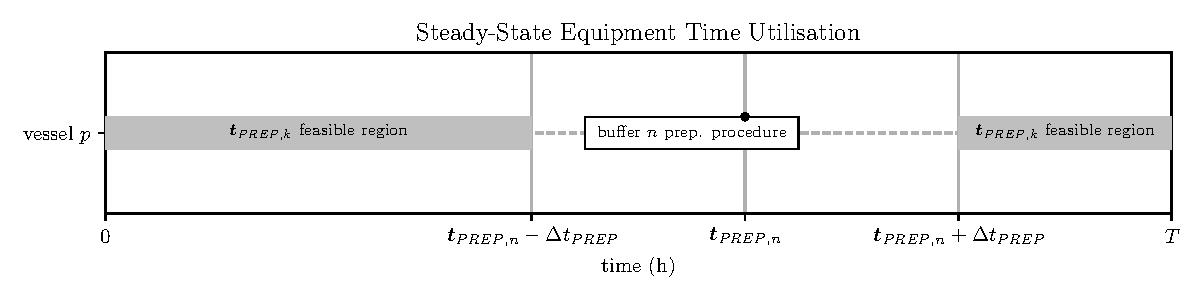
\includegraphics[angle=0,scale=0.7]{./figures/sched1.pdf}
    \caption{Example feasible region for buffer $k$ scheduling}
    \label{fig.sched1}
\end{figure}
Imagine, for instance, that a preparation procedure for buffer $n$ occurs in a
given slot such that it is scheduled well away from the cycle time boundaries.
In such a case, we would envisage two feasible timespans wherein a second
preparation procedure (for, e.g., buffer $k$) may be scheduled in the same
slot.
In terms of the variables defined in 
\hyperref[SS.schedintro]{Section \ref*{SS.schedintro}}, the situation described
above is represented graphically in 
\hyperref[fig.sched1]{Figure \ref*{fig.sched1}}.
The feasible regions may be summarised as follows:
\begin{equation}
    \begin{split}
        \boldsymbol{t}_{\mathit{PREP},k} \ge \boldsymbol{t}_{\mathit{PREP},n} 
        + \Delta t_{\mathit{PREP}} \quad \text{or} \quad 
        \boldsymbol{t}_{\mathit{PREP},k} \le \boldsymbol{t}_{\mathit{PREP},n}
        - \Delta t_{\mathit{PREP}}\\
        \quad \forall n \in N, \enspace \forall k \in N; \; k > n
    \end{split}    
    \label{eq.k0}
\end{equation}
Similar to the approach taken in 
\hyperref[SS.absval]{Section \ref*{SS.absval}}, we can convert the \emph{or}
constraints into \emph{and} constraints by defining an additional binary
variable, $\boldsymbol{v}_{nk}$ and using the \emph{big-M} method. In this
case, $\mathbb{M} = 2T$ is sufficient.
\begin{equation}
    \boldsymbol{v}_{nk} \in \left\{ 0, 1 \right\} \quad \forall n \in N,
    \enspace \forall k \in N; \; k > n
    \label{eq.v}
\end{equation}
\begin{equation}
    \begin{split}
        \begin{alignedat}{2}
            2T \boldsymbol{v}_{nk} + \boldsymbol{t}_{\mathit{PREP},k} &{}\ge{}
            \boldsymbol{t}_{\mathit{PREP},n} {}+{} \Delta t_{\mathit{PREP}}\\
            2T \boldsymbol{v}_{nk} + \boldsymbol{t}_{\mathit{PREP},k} &{}\le{}
            \boldsymbol{t}_{\mathit{PREP},n} {}-{} \Delta t_{\mathit{PREP}}
            {}+{} 2T\\
        \end{alignedat}
    \end{split}
    \quad \forall n \in N, \enspace \forall k \in N; \; k > n
    \label{eq.k1}
\end{equation}
Unfortunately, the above equations do not always hold when the preparation of
one or other of the buffers nears a cycle boundary.
To explain this, \hyperref[fig.sched2]{Figure \ref*{fig.sched2}} (using
\hyperref[fig.sched1]{Figure \ref*{fig.sched1}} as a legend) explores all the
possible cases that must be considered for cyclic scheduling.
\begin{figure}
    \centering
    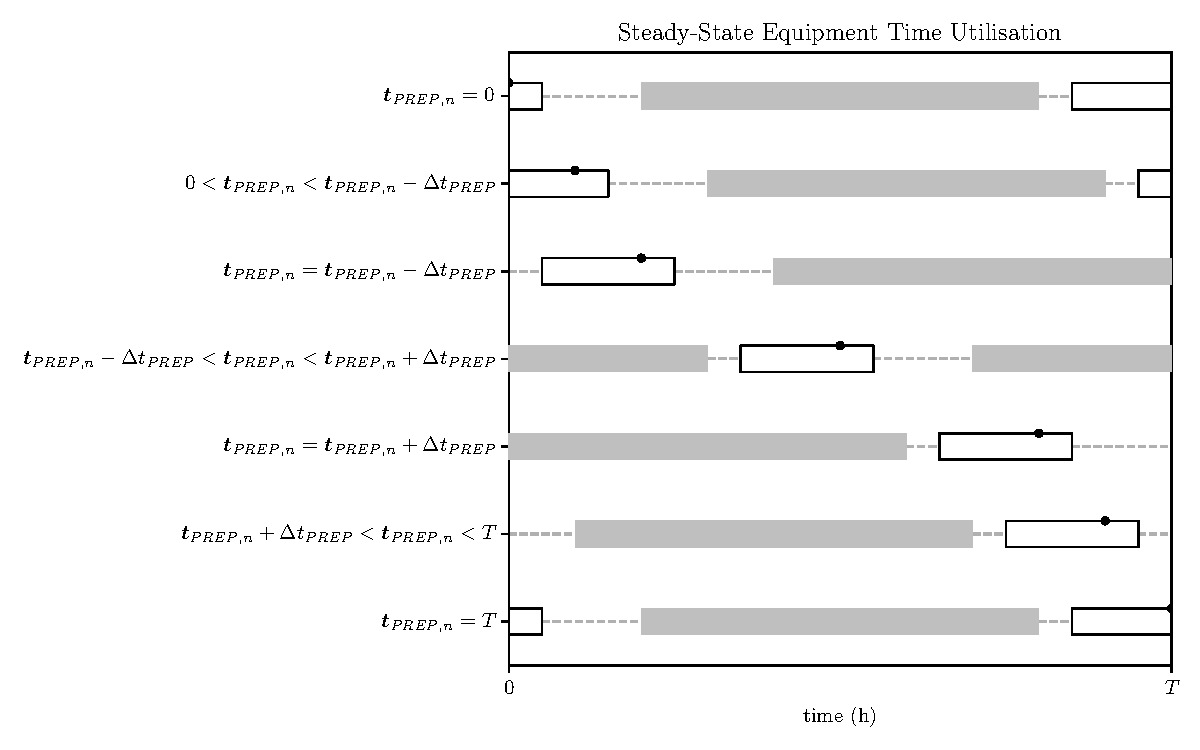
\includegraphics[angle=0,scale=0.7]{./figures/sched2.pdf}
    \caption{All feasible region cases for buffer $k$ scheduling}
    \label{fig.sched2}
\end{figure}
Note that the case shown in \hyperref[fig.sched1]{Figure \ref*{fig.sched1}}, 
i.e.\ the case where
$\left( \boldsymbol{t}_{\mathit{PREP},n} - \Delta t_{\mathit{PREP}} \right) \le 
 \boldsymbol{t}_{\mathit{PREP},k} \le
 \left( \boldsymbol{t}_{\mathit{PREP},n} + \Delta t_{\mathit{PREP}} \right)$
is, in fact, the only case where there are two distinct feasible regions.
For all other cases, there is a single feasible region.  We need to be able to
distinguish between these cases.
Note also that the upper and lower bounds of the feasible region cannot always
be found by adding or subtracting a factor of $\Delta t_{\mathit{PREP}}$
to/from $\boldsymbol{t}_{\mathit{PREP},n}$ respectively, as doing so may result
in values outside the single-cycle range in some instances; we need to add some
logic to prevent this.

The lower bound of the feasible region, $\boldsymbol{t}_{\mathit{LOWER},n}$, is
defined as:
\begin{equation}
    \boldsymbol{t}_{\mathit{LOWER},n} = \boldsymbol{t}_{\mathit{PREP},n} +
    \Delta t_{\mathit{PREP}} - T \boldsymbol{r}_{n} \quad \forall n \in N
    \label{eq.lower1}
\end{equation}
where:
\begin{equation}
    0 \le \boldsymbol{t}_{\mathit{LOWER},n} \le T, \quad 
    \boldsymbol{t}_{\mathit{LOWER},n} \in \mathbb{R}, \enspace \forall n \in N
    \label{eq.lower2}
\end{equation}
and:
\begin{equation}
    \boldsymbol{r}_{n} \in \left\{ 0, 1 \right\} \quad \forall n \in N
    \label{eq.r}
\end{equation}
Similarly, the upper bound of the feasible region, 
$\boldsymbol{t}_{\mathit{UPPER},n}$, is defined as:
\begin{equation}
    \boldsymbol{t}_{\mathit{UPPER},n} = \boldsymbol{t}_{\mathit{PREP},n} -
    \Delta t_{\mathit{PREP}} + T \boldsymbol{s}_{n} \quad \forall n \in N
    \label{eq.upper1}
\end{equation}
where:
\begin{equation}
    0 \le \boldsymbol{t}_{\mathit{UPPER},n} \le T, \quad
    \boldsymbol{t}_{\mathit{LOWER},n} \in \mathbb{R}, \enspace \forall n \in N
    \label{eq.upper2}
\end{equation}
and:
\begin{equation}
    \boldsymbol{s}_{n} \in \left\{ 0, 1 \right\} \quad \forall n \in N
    \label{eq.s}
\end{equation} 
As was the case with \hyperref[eq.tprep]{equation \ref*{eq.tprep}},
equations \ref{eq.lower1} and \ref{eq.upper1} are equalities and so 
$\boldsymbol{t}_{\mathit{LOWER},n}$ and $\boldsymbol{t}_{\mathit{UPPER},n}$
will be replaced by the right hand sides of equations \ref{eq.lower1} and
\ref{eq.upper1} respectively in the final model to reduce complexity.
The new binary variables, $\boldsymbol{r}_{n}$ and $\boldsymbol{s}_{n}$, are
used to ensure values are kept in the single-cycle range, similar to the
function of $\boldsymbol{q}_{n}$ in
\hyperref[eq.tprep]{equation \ref*{eq.tprep}}:
\begin{equation}
    \begin{split}
        \begin{alignedat}{2}
            T \boldsymbol{r}_{n} \le \Delta t_{\mathit{PREP}}
            + \boldsymbol{t}_{\mathit{PREP},n}&\\
            T \boldsymbol{r}_{n} \ge \Delta t_{\mathit{PREP}}
            + \boldsymbol{t}_{\mathit{PREP},n}& - T\\
            \end{alignedat}
        \quad \forall n \in N
    \end{split}
    \label{eq.r1}
\end{equation}
\begin{equation}
    \begin{split}
        \begin{alignedat}{2}
            T \boldsymbol{s}_{n} &\ge \Delta t_{\mathit{PREP}}
            - \boldsymbol{t}_{\mathit{PREP},n}\\
            T \boldsymbol{s}_{n} &\le \Delta t_{\mathit{PREP}} 
            -\boldsymbol{t}_{\mathit{PREP},n} + T
        \end{alignedat}
        \quad \forall n \in N
    \end{split}
    \label{eq.s1}
\end{equation}
Truth tables for equations \ref{eq.r1} and \ref{eq.s1} are given in Tables
\ref{tbl.truthr} and \ref{tbl.truths} respectively.
respectively.
\begin{table}[h!]
    \centering
    \caption{Truth table for $\boldsymbol{r}_{n}$}
    \label{tbl.truthr}
    \begin{tabular}{c | c c | c}
        $t_{\mathit{USE},n} + \Delta t_{\mathit{PREP}}$
        & $\boldsymbol{r}_{n}^{\left( 1 \right)}$
        & $\boldsymbol{r}_{n}^{\left( 2 \right)}$
        & $\boldsymbol{r}_{n} = \boldsymbol{r}_{n}^{\left( 1 \right)} \land
        \boldsymbol{r}_{n}^{\left( 2 \right)}$\\ \hline
        $< T$ & 0 & $\left\{ 0,1 \right\}$ & 0\\
        $T$ & $\left\{ 0,1 \right\}$ & $\left\{ 0,1 \right\}$
            & $\left\{ 0,1 \right\}$\\
        $>T$ & $\left\{ 0,1 \right\}$ & 1 & 1\\
    \end{tabular}
\end{table}
\begin{table}[h!]
    \centering
    \caption{Truth table for $\boldsymbol{s}_{n}$}
    \label{tbl.truths}
    \begin{tabular}{c | c c | c}
        $t_{\mathit{USE},n} - \Delta t_{\mathit{PREP}}$
        & $\boldsymbol{s}_{n}^{\left( 1 \right)}$
        & $\boldsymbol{s}_{n}^{\left( 2 \right)}$
        & $\boldsymbol{s}_{n} = \boldsymbol{s}_{n}^{\left( 1 \right)} \land
        \boldsymbol{s}_{n}^{\left( 2 \right)}$\\ \hline
        $< 0$ & 1 & $\left\{ 0,1 \right\}$ & 1\\
        0 & $\left\{ 0,1 \right\}$ & $\left\{ 0,1 \right\}$
            & $\left\{ 0,1 \right\}$\\
        $> 0$ & $\left\{ 0,1 \right\}$ & 0 & 0\\
    \end{tabular}
\end{table}

As can be seen from \hyperref[fig.sched2]{Figure \ref*{fig.sched2}},
the feasible region, when contiguous in the single-cycle window,
is bounded below by $\boldsymbol{t}_{\mathit{LOWER},n}$ and above by
$\boldsymbol{t}_{\mathit{UPPER},n}$, giving rise to the following two
constraints:
\begin{equation}
    \begin{split}
        \boldsymbol{t}_{\mathit{PREP},k} 
        \ge \boldsymbol{t}_{\mathit{LOWER},n}\\
        \boldsymbol{t}_{\mathit{PREP},k} 
        \le \boldsymbol{t}_{\mathit{UPPER},n}
    \end{split}
    \quad \forall n \in N, \enspace \forall k \in N; \; k > n
    \label{eq.k2}
\end{equation}
Recall that constraints on $\boldsymbol{t}_{\mathit{PREP},k}$ were defined in
\hyperref[eq.k1]{equation \ref*{eq.k1}}, for the case where there were two
distinct feasible regions in the cycle.
In \hyperref[eq.k2]{equation \ref*{eq.k2}} above, we have now detailed
constraints on $\boldsymbol{t}_{\mathit{PREP},k}$ for the cases where there is
a single, contiguous feasible region in the cycle.
All that is left to do is to define another binary variable that selects
between these two sets of constraints.
By looking at \hyperref[fig.sched2]{Figure \ref*{fig.sched2}}, it can be seen
that we are only interested in applying the constraints in 
\hyperref[eq.k1]{equation \ref*{eq.k1}} when both
$\boldsymbol{t}_{\mathit{UPPER},n} < \boldsymbol{t}_{\mathit{PREP},n}$ and
$\boldsymbol{t}_{\mathit{LOWER},n} > \boldsymbol{t}_{\mathit{PREP},n}$, i.e.\
when both $\boldsymbol{r}_{n} = 0$ and $\boldsymbol{s}_{n} = 0$.
In all other cases, we wish to apply the constraints in
\hyperref[eq.k2]{equation \ref*{eq.k2}}.
We therefore define a new binary variable, $\boldsymbol{u}_{n}$, where 
$\boldsymbol{u}_{n} = 0$ iff $\boldsymbol{r}_{n} = 0$ and 
$\boldsymbol{s}_{n} = 0$.
\begin{equation}
    \boldsymbol{u}_{n} \in \left\{ 0, 1 \right\} \quad \forall n \in N
    \label{eq.u}
\end{equation}
\begin{equation}
    \begin{split}
        \begin{alignedat}{8}
            \boldsymbol{u}_{n} &\le &&\boldsymbol{r}_{n}
            && {}+{} &&\boldsymbol{s}_{n}\\
            \boldsymbol{u}_{n} &\ge \tfrac{1}{2} &&\boldsymbol{r}_{n}
            && {}+{} \tfrac{1}{2} &&\boldsymbol{s}_{n}\\
        \end{alignedat}
        \quad \forall n \in N
    \end{split}
    \label{eq.u1}
\end{equation}
A truth table for \hyperref[eq.u1]{equation \ref*{eq.u1}} is given in 
\hyperref[tbl.truthu]{Table \ref*{tbl.truthu}}.
\begin{table}[h!]
    \centering
    \caption{Truth table for $\boldsymbol{u}_{n}$}
    \label{tbl.truthu}
    \begin{tabular}{c c | c c | c}
        $\boldsymbol{r}_{n}$ & $\boldsymbol{s}_{n}$ &
        $\boldsymbol{u}_{n}^{\left( 1 \right)}$ &
        $\boldsymbol{u}_{n}^{\left( 2 \right)}$ &
        $\boldsymbol{u}_{n} = \boldsymbol{u}_{n}^{\left( 1 \right)}
            \land \boldsymbol{u}_{n}^{\left( 2 \right)}
        $\\ \hline
        0 & 0 & 0 & $\left\{ 0,1 \right\}$ & 0\\
        0 & 1 & $\left\{ 0,1 \right\}$ & 1 & 1\\
        1 & 0 & $\left\{ 0,1 \right\}$ & 1 & 1\\
        1 & 1 & $\left\{ 0,1 \right\}$ & 1 & 1\\
    \end{tabular}
\end{table}
With the definition of $\boldsymbol{u}_{n}$, a unified set of inequalities can
be written which describe the scheduling of buffers prepared in the same slot.
Once again, the \emph{big-M} method is employed, with $\mathbb{M} = 2T$.
\begin{equation}
    \begin{split}
        \begin{alignedat}{10}
            \boldsymbol{t}_{\mathit{PREP},k}
            &\le \boldsymbol{t}_{\mathit{PREP},n}
            - \Delta t_{\mathit{PREP}} {}+{} & 2T &\boldsymbol{u}_{n}
            {}-{} & 2T &\boldsymbol{v}_{nk} & {}+{} 2T&\\
            \boldsymbol{t}_{\mathit{PREP},k}
            &\ge \boldsymbol{t}_{\mathit{PREP},n}
            + \Delta t_{\mathit{PREP}} {}-{} & 2T &\boldsymbol{u}_{n}
            {}-{} & 2T &\boldsymbol{v}_{nk}&\\
            \boldsymbol{t}_{\mathit{PREP},k}
            &\le \boldsymbol{t}_{\mathit{PREP},n}
            - \Delta t_{\mathit{PREP}} {}-{} & 2T &\boldsymbol{u}_{n}
            {}+{} & T &\boldsymbol{r}_{n} & {}+{} 2T&\\
            \boldsymbol{t}_{\mathit{PREP},k}
            &\ge \boldsymbol{t}_{\mathit{PREP},n}
            + \Delta t_{\mathit{PREP}} {}+{} & 2T &\boldsymbol{u}_{n}
            {}-{} & T &\boldsymbol{s}_{n} & {}-{} 2T&\\
            &\forall n \in N, \enspace \forall k \in N; \; k > n
            \end{alignedat}            
    \end{split}
    \label{eq.k4}
\end{equation}

\subsection{Preparation Scheduling}\label{SS.prepsched}
The constraints in \hyperref[eq.k4]{equation \ref*{eq.k4}} are only valid for
the case where buffers $n$ and $k$ are prepared in the same slot.
Recall that we defined a variable, $\boldsymbol{a}_{nk}$, which indicated if
this is the case.
Accordingly, the final preparation scheduling constraint is a modification of
\hyperref[eq.k4]{equation \ref*{eq.k4}} which uses the \emph{big-M} method,
with $\mathbb{M} = 2T$, to disable all of the constraints when
$\boldsymbol{a}_{nk} = 0$.
The final preparation constraint is given in equation
\hyperref[eq.k5]{equation \ref*{eq.k5}} below. 
\begin{equation}
    \begin{split}
        \begin{alignedat}{14}
            \boldsymbol{t}_{\mathit{PREP},k}
            &\le \boldsymbol{t}_{\mathit{PREP},n}
            - \Delta t_{\mathit{PREP}} {}-{} & 2T &\boldsymbol{a}_{nk}
            {}+{} & 2T &\boldsymbol{u}_{n}
            {}-{} & 2T &\boldsymbol{v}_{nk} & {}+{} 4T&\\
            \boldsymbol{t}_{\mathit{PREP},k}
            &\ge \boldsymbol{t}_{\mathit{PREP},n}
            + \Delta t_{\mathit{PREP}} {}+{} & 2T &\boldsymbol{a}_{nk}
            {}-{} & 2T &\boldsymbol{u}_{n}
            {}-{} & 2T &\boldsymbol{v}_{nk} & {}-{} 2T&\\
            \boldsymbol{t}_{\mathit{PREP},k}
            &\le \boldsymbol{t}_{\mathit{PREP},n}
            - \Delta t_{\mathit{PREP}} {}-{} & 2T &\boldsymbol{a}_{nk}
            {}-{} & 2T &\boldsymbol{u}_{n}
            {}+{} & T &\boldsymbol{r}_{n} & {}+{} 4T&\\
            \boldsymbol{t}_{\mathit{PREP},k}
            &\ge \boldsymbol{t}_{\mathit{PREP},n}
            + \Delta t_{\mathit{PREP}} {}+{} & 2T &\boldsymbol{a}_{nk}
            {}+{} & 2T &\boldsymbol{u}_{n}
            {}-{} & T &\boldsymbol{s}_{n} & {}-{} 4T&\\
            &\forall n \in N, \enspace \forall k \in N; \; k > n
            \end{alignedat}            
    \end{split}
    \label{eq.k5}
\end{equation}

A truth table for \hyperref[eq.k5]{equation \ref*{eq.k5}} is given in
\hyperref[tbl.truthsched]{Table \ref*{tbl.truthsched}}, with $\ast$ denoting
the set $\left\{0,1\right\}$.
\begin{table}[h!]
    \centering
    \caption{Truth table for equation \ref{eq.k5}}
    \label{tbl.truthsched}
    \begin{tabular}{c c c c c | c}
        $\boldsymbol{a}_{nk}$ & $\boldsymbol{u}_{n}$ & $\boldsymbol{v}_{n}$
        & $\boldsymbol{r}_{n}$ & $\boldsymbol{s}_{n}$
        & $\boldsymbol{t}_{\mathit{PREP},k} = \bullet$\\\hline
        0 & $\ast$ & $\ast$ & $\ast$ & $\ast$ 
        & (no active scheduling constraints)\\
        1 & 0 & 0 & $\ast$ & $\ast$
        & $\bullet \ge \boldsymbol{t}_{\mathit{PREP},n} 
           + \Delta t_{\mathit{PREP}}$\\
        1 & 0 & 1 & $\ast$ & $\ast$ 
        & $\bullet \le \boldsymbol{t}_{\mathit{PREP},n} 
           - \Delta t_{\mathit{PREP}}$\\
        1 & 1 & $\ast$ & 0 & 0 
        & $\boldsymbol{t}_{\mathit{PREP},n} + \Delta t_{\mathit{PREP}}
           \le \bullet \le \boldsymbol{t}_{\mathit{PREP},n} 
           - \Delta t_{\mathit{PREP}}$\\
        1 & 1 & $\ast$ & 0 & 1 
        & $\boldsymbol{t}_{\mathit{PREP},n} + \Delta t_{\mathit{PREP}} - T
           \le \bullet \le \boldsymbol{t}_{\mathit{PREP},n}
           - \Delta t_{\mathit{PREP}}$\\
        1 & 1 & $\ast$ & 1 & 0 
        & $\boldsymbol{t}_{\mathit{PREP},n} + \Delta t_{\mathit{PREP}}
           \le \bullet \le \boldsymbol{t}_{\mathit{PREP},n}
           - \Delta t_{\mathit{PREP}} + T$\\
        1 & 1 & $\ast$ & 1 & 1 
        & $\boldsymbol{t}_{\mathit{PREP},n} + \Delta t_{\mathit{PREP}} - T
           \le \bullet \le \boldsymbol{t}_{\mathit{PREP},n}
           - \Delta t_{\mathit{PREP}} + T$\\
    \end{tabular}
\end{table}


\subsection{Complete Model Summary}\label{SS.completesummary}

The complete model is summarised below.
The constraint equations have been rearranged so that variables are on the left
hand side and constants are on the right. 

Minimise:
\begin{equation}
    \boldsymbol{Z} = \sum_{m \in M} \sum_{p \in P} c_m \boldsymbol{y}_{mp}
    \tag{\ref{eq.objfn}}
\end{equation}
Subject to:
\begin{equation}
    \sum_{p \in P} \boldsymbol{x}_{np} = 1 \quad \forall n \in N
    \tag{\ref{eq.constr1}}
\end{equation}
\begin{equation}
    \sum_{m \in M} \boldsymbol{y}_{mp} \le 1 \quad \forall p \in P
    \tag{\ref{eq.constr2}}
\end{equation}
\begin{equation}
    U_{n} \boldsymbol{x}_{np} - \sum_{m \in M} V_{m} \boldsymbol{y}_{mp} \le 0
    \quad \forall n \in N, \enspace \forall p \in P
    \tag{\ref{eq.constr3a}}
\end{equation}
\begin{equation}
    V_{\mathit{MAX}} \boldsymbol{x}_{np} + f_{\mathit{MINFILL}} \sum_{m \in M}
    V_{m} \boldsymbol{y}_{mp} \le U_{n} + V_{\mathit{MAX}} \quad \forall n \in
    N, \enspace \forall p \in P
    \tag{\ref{eq.constr3b}}
\end{equation}
\begin{equation}
    \Delta t_{\mathit{PREP}} \sum_{n \in N} \boldsymbol{x}_{np} \le
    f_{\mathit{UTIL}} T \quad \forall p \in P
    \tag{\ref{eq.constr4}}
\end{equation}
%new equations
\begin{equation}
    \begin{aligned}
        \boldsymbol{z}_{n} \le T - \Delta t_{\mathit{HOLD,PRE}}
        - \Delta t_{\mathit{TRANSFER}} - \Delta t_{\mathit{USE},n}
        - \Delta t_{\mathit{HOLD,POST}}\\
        \quad \forall n \in N
    \end{aligned}
    \tag{\ref{eq.z1}}
\end{equation}
\begin{equation}
    \begin{split}
        \begin{alignedat}{11}
            2&\boldsymbol{w}_{nkp} {}-{} &&\boldsymbol{x}_{np}
            {}-{} && \boldsymbol{x}_{kp} {}&&\le{} &{}-{} 2\\
            &\boldsymbol{w}_{nkp} {}-{} &&\boldsymbol{x}_{np}
            {}-{} && \boldsymbol{x}_{kp} {}&&\ge{} &{}-{} 1\\
        \end{alignedat}
    \end{split}
    \quad
    \begin{split}
        \forall n \in N, \enspace \forall k \in N; \; k > n, \enspace 
        \forall p \in P
    \end{split}
    \tag{\ref{eq.w1}}
\end{equation}
\begin{equation}
    \begin{split}
        \begin{alignedat}{2}
            T \boldsymbol{q}_{n} - \boldsymbol{z}_{n} &\ge
            - t_{\mathit{USE},n}\\
            T \boldsymbol{q}_{n} - \boldsymbol{z}_{n} &\le
            - t_{\mathit{USE},n} + T\\
        \end{alignedat}
    \end{split}
    \quad \forall n \in N
    \tag{\ref{eq.q1}}
\end{equation}
\begin{equation}
    \begin{split}
        \begin{alignedat}{2}
            -T \boldsymbol{q}_{n} + T \boldsymbol{r}_{n} + \boldsymbol{z}_{n}
            &\le t_{\mathit{USE},n} + \Delta t_{\mathit{PREP}}\\
            -T \boldsymbol{q}_{n} + T \boldsymbol{r}_{n} + \boldsymbol{z}_{n}
            &\ge t_{\mathit{USE},n} + \Delta t_{\mathit{PREP}} - T\\
            \end{alignedat}
        \quad \forall n \in N
    \end{split}
    \label{eq.r2}
\end{equation}
\begin{equation}
    \begin{split}
        \begin{alignedat}{2}
            T \boldsymbol{q}_{n} + T \boldsymbol{s}_{n} - \boldsymbol{z}_{n}
            &\le -t_{\mathit{USE},n} + \Delta t_{\mathit{PREP}}\\
            T \boldsymbol{q}_{n} + T \boldsymbol{s}_{n} - \boldsymbol{z}_{n}
            &\ge -t_{\mathit{USE},n} + \Delta t_{\mathit{PREP}} + T\\
            \end{alignedat}
        \quad \forall n \in N
    \end{split}
    \label{eq.s2}
\end{equation}
\begin{equation}
    \begin{split}
        \begin{alignedat}{8}
            &&\boldsymbol{r}_{n} && {}+{} &&\boldsymbol{s}_{n} && {}-{} 
            &&\boldsymbol{u}_{n} &\ge 0\\
            &&\boldsymbol{r}_{n} && {}+{} &&\boldsymbol{s}_{n} && {}-{} 
            &2&\boldsymbol{u}_{n} &\le 0\\
        \end{alignedat}
        \quad \forall n \in N
    \end{split}
    \tag{\ref{eq.u1}}
\end{equation}
\begin{equation}
    \begin{split}
        \begin{aligned}
            T \boldsymbol{q}_{k} - T \boldsymbol{q}_{n} + 2T \boldsymbol{u}_{n} 
            + 2T \boldsymbol{v}_{nk} - 2T \sum_{p \in P} \boldsymbol{w}_{nkp} 
            - \boldsymbol{z}_{k} + \boldsymbol{z}_{n}\\
            \ge t_{\mathit{USE},n} - t_{\mathit{USE},k}
            + \Delta t_{\mathit{PREP}} - 2T
        \end{aligned}\\
        \begin{aligned}
            T \boldsymbol{q}_{k} - T \boldsymbol{q}_{n} - 2T \boldsymbol{u}_{n} 
            + 2T \boldsymbol{v}_{nk} + 2T \sum_{p \in P} \boldsymbol{w}_{nkp} 
            - \boldsymbol{z}_{k} + \boldsymbol{z}_{n}\\
            \ge t_{\mathit{USE},n} - t_{\mathit{USE},k}
            - \Delta t_{\mathit{PREP}} + 4T
        \end{aligned}\\
        \begin{aligned}
            T \boldsymbol{q}_{k} - T \boldsymbol{q}_{n} - T \boldsymbol{r}_{n}
            + 2T \boldsymbol{u}_{n} + 2T \sum_{p \in P} \boldsymbol{w}_{nkp} 
            - \boldsymbol{z}_{k} + \boldsymbol{z}_{n}\\
            \ge t_{\mathit{USE},n} - t_{\mathit{USE},k}
            - \Delta t_{\mathit{PREP}} + 4T
        \end{aligned}\\
        \begin{aligned}
            T \boldsymbol{q}_{k} - T \boldsymbol{q}_{n} + T \boldsymbol{s}_{n}
            - 2T \boldsymbol{u}_{n} - 2T \sum_{p \in P} \boldsymbol{w}_{nkp} 
            - \boldsymbol{z}_{k} + \boldsymbol{z}_{n}\\
            \ge t_{\mathit{USE},n} - t_{\mathit{USE},k}
            + \Delta t_{\mathit{PREP}} - 4T
        \end{aligned}\\
        \begin{aligned}
            \forall n \in N, \enspace \forall k \in N; \; k > n
        \end{aligned}\\
    \end{split}
    \label{eq.k6}
\end{equation}
Where:
\begin{equation}
    \boldsymbol{q}_{n} \in \left\{0, 1\right\} \quad \forall n \in N
    \tag{\ref{eq.q}}
\end{equation}
\begin{equation}
    \boldsymbol{r}_{n} \in \left\{ 0, 1 \right\} \quad \forall n \in N
    \tag{\ref{eq.r}}
\end{equation}
\begin{equation}
    \boldsymbol{s}_{n} \in \left\{ 0, 1 \right\} \quad \forall n \in N
    \tag{\ref{eq.s}}
\end{equation} 
\begin{equation}
    \boldsymbol{u}_{n} \in \left\{ 0, 1 \right\} \quad \forall n \in N
    \tag{\ref{eq.u}}
\end{equation}
\begin{equation}
    \boldsymbol{v}_{nk} \in \left\{ 0, 1 \right\} \quad \forall n \in N,
    \enspace \forall k \in N; \; k > n
    \tag{\ref{eq.v}}
\end{equation}
\begin{equation}
    \boldsymbol{w}_{nkp} \in \left\{ 0, 1 \right\} \quad \forall n \in N, 
    \enspace \forall k \in N; \; k > n, \enspace \forall p \in P
    \tag{\ref{eq.w}}
\end{equation}
\begin{equation}
    \boldsymbol{x}_{np} \in \left\{ 0, 1 \right\} \quad \forall n \in N,
    \enspace \forall p \in P
    \tag{\ref{eq.x}}
\end{equation}
\begin{equation}
    \boldsymbol{y}_{mp} \in \left\{ 0, 1 \right\} \quad \forall m \in M,
    \enspace \forall p \in P
    \tag{\ref{eq.y}}
\end{equation}
\begin{equation}
    \Delta t_{\mathit{HOLD,MIN}} \le \boldsymbol{z}_{n} \le 
    \Delta t_{\mathit{HOLD,MAX}}; \quad
    \boldsymbol{z}_{n} \in \mathbb{R} \quad \forall n \in N
    \tag{\ref{eq.z}}
\end{equation}

Note that variables $\boldsymbol{a}_{nk}$, $\boldsymbol{t}_{\mathit{PREP},n}$,
$\boldsymbol{t}_{\mathit{PREP},k}$, $\boldsymbol{t}_{\mathit{LOWER},n}$ and
$\boldsymbol{t}_{\mathit{UPPER},n}$ are not required in the model. Values for
these variables can be obtained, post solution, by applying equations
\ref{eq.a1}, \ref{eq.tprep}, \ref{eq.tprep} (replacing $n$ with $k$),
\ref{eq.lower1} and \ref{eq.upper1} respectively.

\section{Further Optimisation}\label{S.secondary}

\subsection{Goal programming}\label{SS.goal}
The complete model summarised in 
\hyperref[SS.completesummary]{Section \ref*{SS.completesummary}} may be solved
to give the required number of vessels that correspond to the minimum cost.
As was alluded to in \hyperref[S.outputdata]{Section \ref*{S.outputdata}},
there may be many possible feasible solutions that correspond to this minimum
cost and would yield the same set of vessels (though the selected preparation
vessels may not necessarily be used to prepare the same buffers).
Thus, there may be many ways to represent an optimal process schedule.

If, for example, the data described in
\hyperref[C.data]{Chapter \ref*{C.data}} were to be used as an input to the
complete model, a feasible optimal schedule, such as that shown in
\hyperref[fig.primary]{Figure \ref*{fig.primary}} may be generated.
Note that this is identical to \hyperref[fig.etu1]{Figure \ref*{fig.etu1}}
discussed in \hyperref[C.data]{Chapter \ref*{C.data}},
but it is also included here to illustrate the effects of goal programming.

\begin{figure}
    \centering
    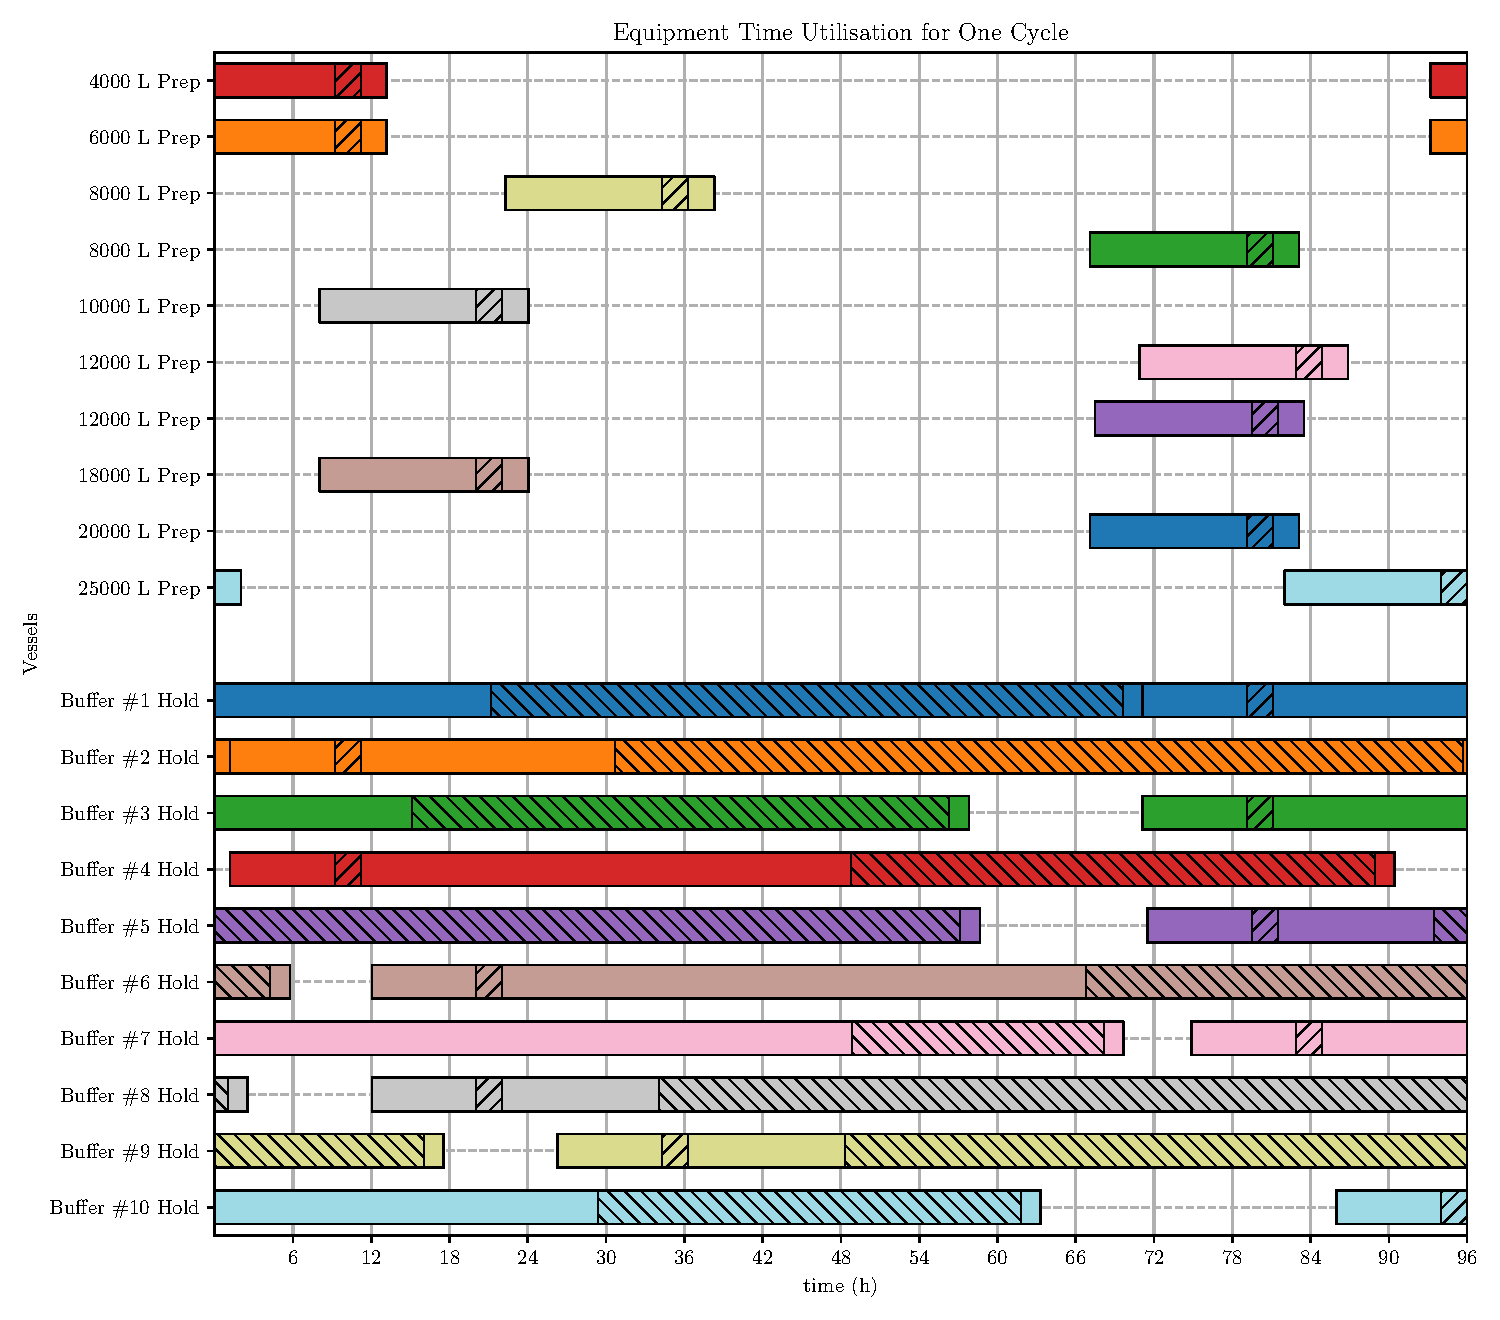
\includegraphics[angle=0,scale=0.55]{./figures/plot1.pdf}
    \caption{Large-scale example -- primary objective}
    \label{fig.primary}
\end{figure}
Note that the solution requires four vessels, with sizes
\SI{2000}{\litre}, \SI{8000}{\litre}, \SI{25000}{\litre} and \SI{30000}{\litre}
respectively.  
Recall that one of our decision variables is $\boldsymbol{z}_{n}$, the buffer
hold duration.
In \hyperref[fig.primary]{Figure \ref*{fig.primary}}, we can see that Buffer
\#2 is scheduled such that its hold procedure is bottlenecked, i.e.\ the start
of the hold procedure for a given batch coincides precisely with the end of the
hold procedure for the previous batch.
For this buffer, it can also be seen that there exists some free time after
its preparation procedure.

Delaying the preparation of Buffer \#2 by e.g.\ three hours would
also give an optimal solution, with the vessel selection unchanged and would
prevent the hold procedure for Buffer \#2 from being bottlenecked.
There exists sufficient free time in the \SI{8000}{\litre} vessel to do this.
Note that delaying a preparation by some amount $\delta$ is equivalent to 
reducing $\boldsymbol{z}_{n}$ by $\delta$.
Recall also that $\boldsymbol{z}_{n}$ has a lower bound, 
$\Delta t_{\mathit{HOLD,MIN}}$.

In terms of visualising a realistic schedule, it is desirable to minimise the
hold durations, i.e.\ we wish to define a new objective function, to be
minimised:
\begin{equation}
    \boldsymbol{Y} = \sum_{n \in N} \boldsymbol{z}_{n} \quad \forall n \in N
    \label{eq.objfn2}
\end{equation}
Note that we want to maintain the original optimum objective function value,
i.e.\ we define:
\begin{equation}
    Z^{\prime} = \min \boldsymbol{Z}
    \label{eq.Zprime}
\end{equation}
In \hyperref[eq.Zprime]{equation \ref*{eq.Zprime}}, $Z^{\prime}$ is the optimal objective function value
obtained by solving the complete model.
Note that $Z^{\prime}$ is not bolded, as it is treated as a constant parameter
in our second-pass model.
The complete model is then re-run with the original objective function replaced
by the new objective, $\min \boldsymbol{Y}$, with the following constraint
added:
\begin{equation}
    \sum_{m \in M} \sum_{p \in P} c_m \boldsymbol{y}_{mp} = Z^{\prime}
    \label{eq.constr10}
\end{equation}
\begin{figure}
    \centering
    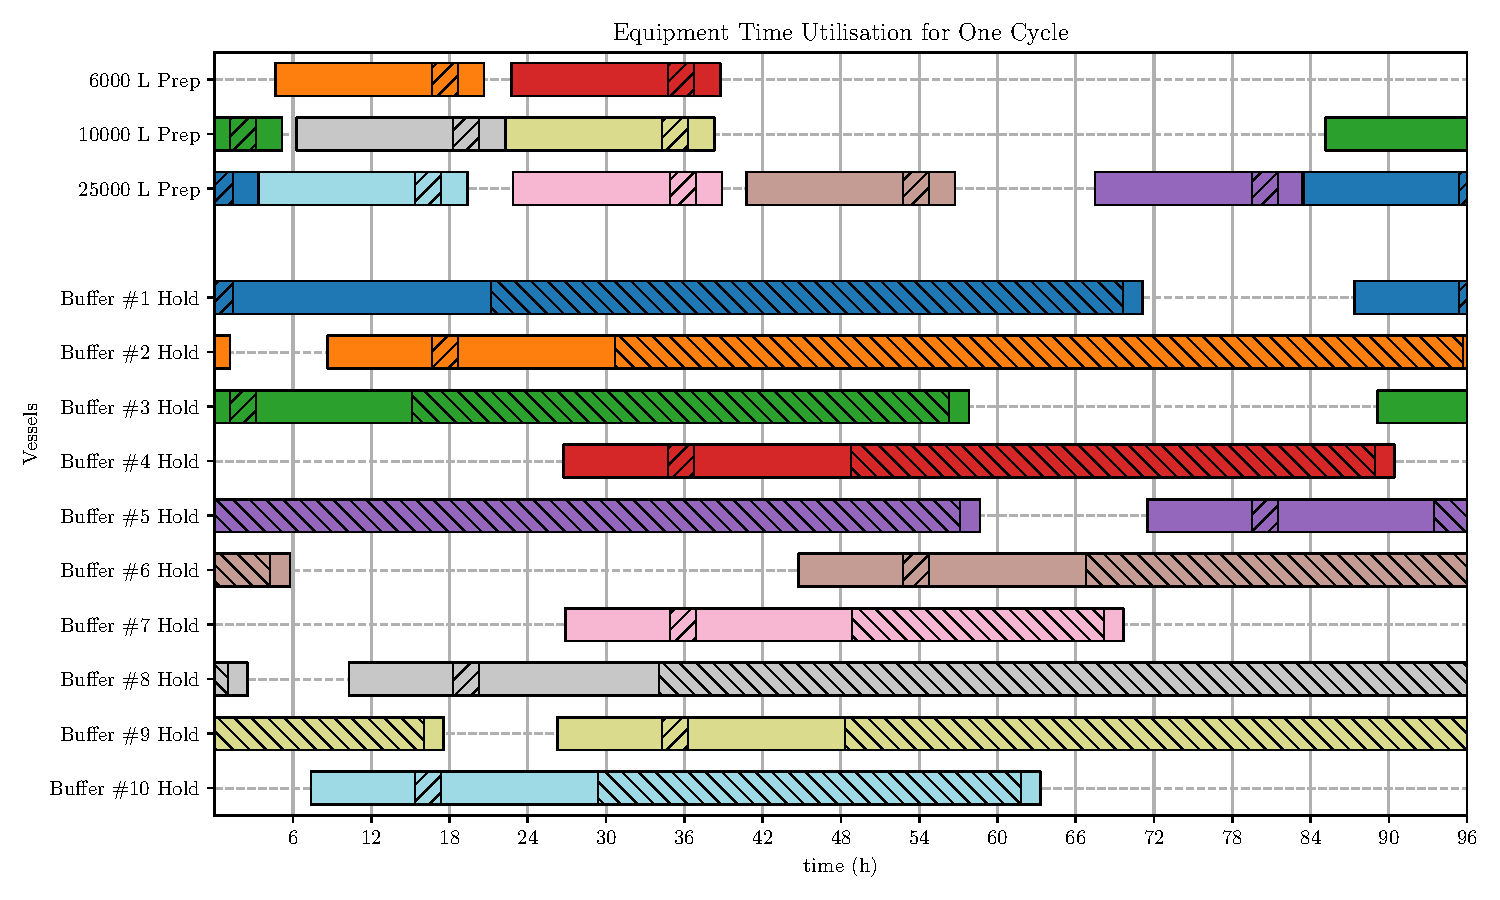
\includegraphics[angle=0,scale=0.55]{./figures/plot2.pdf}
    \caption{Large-scale example -- secondary objective}
    \label{fig.secondary}
\end{figure}

Implementing the secondary goal programming model on the same data-set yields
the plot shown in \hyperref[fig.secondary]{Figure \ref*{fig.secondary}}
Note that the buffer hold procedure for Buffer \#2 is no longer bottlenecked.
We can also see that the hold times for Buffers \#1, \#6, \#7 and \#12 have
all decreased, but the hold time for buffer \#4 has increased.
Overall, there has been a reduction in total hold time, which was our aim.
Note also that, although the same preparation vessels are selected (i.e.\ the
same minimal cost is obtained), some buffers are now prepared in different
vessels to those originally assigned.
For example, in the original result, Buffers \#1 and \#6 were prepared in the
\SI{25000}{\litre} vessel and with the secondary goal added, they are now
prepared in the \SI{30000}{\litre} vessel.
Conversely, preparation of Buffer \#7 shifts from the \SI{30000}{\litre} vessel
to the \SI{25000}{\litre} vessel.

\subsection{Secondary Model Summary}\label{SS.model2summary}

The secondary model is summarised below:

Minimise:
\begin{equation}
    \boldsymbol{Y} = \sum_{n \in N} \boldsymbol{z}_{n} \quad \forall n \in N
    \tag{\ref{eq.objfn2}}
\end{equation}
Subject to:
\begin{equation}
    \sum_{p \in P} \boldsymbol{x}_{np} = 1 \quad \forall n \in N
    \tag{\ref{eq.constr1}}
\end{equation}
\begin{equation}
    \sum_{m \in M} \boldsymbol{y}_{mp} \le 1 \quad \forall p \in P
    \tag{\ref{eq.constr2}}
\end{equation}
\begin{equation}
    U_{n} \boldsymbol{x}_{np} - \sum_{m \in M} V_{m} \boldsymbol{y}_{mp} \le 0
    \quad \forall n \in N, \enspace \forall p \in P
    \tag{\ref{eq.constr3a}}
\end{equation}
\begin{equation}
    V_{\mathit{MAX}} \boldsymbol{x}_{np} + f_{\mathit{MINFILL}} \sum_{m \in M}
    V_{m} \boldsymbol{y}_{mp} \le U_{n} + V_{\mathit{MAX}} \quad \forall n \in
    N, \enspace \forall p \in P
    \tag{\ref{eq.constr3b}}
\end{equation}
\begin{equation}
    \Delta t_{\mathit{PREP}} \sum_{n \in N} \boldsymbol{x}_{np} \le
    f_{\mathit{UTIL}} T \quad \forall p \in P
    \tag{\ref{eq.constr4}}
\end{equation}
%new equations
\begin{equation}
    \begin{aligned}
        \boldsymbol{z}_{n} \le T - \Delta t_{\mathit{HOLD,PRE}}
        - \Delta t_{\mathit{TRANSFER}} - \Delta t_{\mathit{USE},n}
        - \Delta t_{\mathit{HOLD,POST}}\\
        \quad \forall n \in N
    \end{aligned}
    \tag{\ref{eq.z1}}
\end{equation}
\begin{equation}
    \begin{split}
        \begin{alignedat}{11}
            2&\boldsymbol{w}_{nkp} {}-{} &&\boldsymbol{x}_{np}
            {}-{} && \boldsymbol{x}_{kp} {}&&\le{} &{}-{} 2\\
            &\boldsymbol{w}_{nkp} {}-{} &&\boldsymbol{x}_{np}
            {}-{} && \boldsymbol{x}_{kp} {}&&\ge{} &{}-{} 1\\
        \end{alignedat}
    \end{split}
    \quad
    \begin{split}
        \forall n \in N, \enspace \forall k \in N; \; k > n, \enspace 
        \forall p \in P
    \end{split}
    \tag{\ref{eq.w1}}
\end{equation}
\begin{equation}
    \begin{split}
        \begin{alignedat}{2}
            T \boldsymbol{q}_{n} - \boldsymbol{z}_{n} &\ge
            - t_{\mathit{USE},n}\\
            T \boldsymbol{q}_{n} - \boldsymbol{z}_{n} &\le
            - t_{\mathit{USE},n} + T\\
        \end{alignedat}
    \end{split}
    \quad \forall n \in N
    \tag{\ref{eq.q1}}
\end{equation}
\begin{equation}
    \begin{split}
        \begin{alignedat}{2}
            -T \boldsymbol{q}_{n} + T \boldsymbol{r}_{n} + \boldsymbol{z}_{n}
            &\le t_{\mathit{USE},n} + \Delta t_{\mathit{PREP}}\\
            -T \boldsymbol{q}_{n} + T \boldsymbol{r}_{n} + \boldsymbol{z}_{n}
            &\ge t_{\mathit{USE},n} + \Delta t_{\mathit{PREP}} - T\\
            \end{alignedat}
        \quad \forall n \in N
    \end{split}
    \tag{\ref{eq.r2}}
\end{equation}
\begin{equation}
    \begin{split}
        \begin{alignedat}{2}
            T \boldsymbol{q}_{n} + T \boldsymbol{s}_{n} - \boldsymbol{z}_{n}
            &\le -t_{\mathit{USE},n} + \Delta t_{\mathit{PREP}}\\
            T \boldsymbol{q}_{n} + T \boldsymbol{s}_{n} - \boldsymbol{z}_{n}
            &\ge -t_{\mathit{USE},n} + \Delta t_{\mathit{PREP}} + T\\
            \end{alignedat}
        \quad \forall n \in N
    \end{split}
    \tag{\ref{eq.s2}}
\end{equation}
\begin{equation}
    \begin{split}
        \begin{alignedat}{8}
            &&\boldsymbol{r}_{n} && {}+{} &&\boldsymbol{s}_{n} && {}-{} 
            &&\boldsymbol{u}_{n} &\ge 0\\
            &&\boldsymbol{r}_{n} && {}+{} &&\boldsymbol{s}_{n} && {}-{} 
            &2&\boldsymbol{u}_{n} &\le 0\\
        \end{alignedat}
        \quad \forall n \in N
    \end{split}
    \tag{\ref{eq.u1}}
\end{equation}
\begin{equation}
    \begin{split}
        \begin{aligned}
            T \boldsymbol{q}_{k} - T \boldsymbol{q}_{n} + 2T \boldsymbol{u}_{n} 
            + 2T \boldsymbol{v}_{nk} - 2T \sum_{p \in P} \boldsymbol{w}_{nkp} 
            - \boldsymbol{z}_{k} + \boldsymbol{z}_{n}\\
            \ge t_{\mathit{USE},n} - t_{\mathit{USE},k}
            + \Delta t_{\mathit{PREP}} - 2T
        \end{aligned}\\
        \begin{aligned}
            T \boldsymbol{q}_{k} - T \boldsymbol{q}_{n} - 2T \boldsymbol{u}_{n} 
            + 2T \boldsymbol{v}_{nk} + 2T \sum_{p \in P} \boldsymbol{w}_{nkp} 
            - \boldsymbol{z}_{k} + \boldsymbol{z}_{n}\\
            \ge t_{\mathit{USE},n} - t_{\mathit{USE},k}
            - \Delta t_{\mathit{PREP}} + 4T
        \end{aligned}\\
        \begin{aligned}
            T \boldsymbol{q}_{k} - T \boldsymbol{q}_{n} - T \boldsymbol{r}_{n}
            + 2T \boldsymbol{u}_{n} + 2T \sum_{p \in P} \boldsymbol{w}_{nkp} 
            - \boldsymbol{z}_{k} + \boldsymbol{z}_{n}\\
            \ge t_{\mathit{USE},n} - t_{\mathit{USE},k}
            - \Delta t_{\mathit{PREP}} + 4T
        \end{aligned}\\
        \begin{aligned}
            T \boldsymbol{q}_{k} - T \boldsymbol{q}_{n} + T \boldsymbol{s}_{n}
            - 2T \boldsymbol{u}_{n} - 2T \sum_{p \in P} \boldsymbol{w}_{nkp} 
            - \boldsymbol{z}_{k} + \boldsymbol{z}_{n}\\
            \ge t_{\mathit{USE},n} - t_{\mathit{USE},k}
            + \Delta t_{\mathit{PREP}} - 4T
        \end{aligned}\\
        \begin{aligned}
            \forall n \in N, \enspace \forall k \in N; \; k > n
        \end{aligned}\\
    \end{split}
    \tag{\ref{eq.k6}}
\end{equation}
\begin{equation}
    \sum_{m \in M} \sum_{p \in P} c_m \boldsymbol{y}_{mp} = Z^{\prime}
    \tag{\ref{eq.constr10}}
\end{equation}
Where:
\begin{equation}
    \boldsymbol{q}_{n} \in \left\{0, 1\right\} \quad \forall n \in N
    \tag{\ref{eq.q}}
\end{equation}
\begin{equation}
    \boldsymbol{r}_{n} \in \left\{ 0, 1 \right\} \quad \forall n \in N
    \tag{\ref{eq.r}}
\end{equation}
\begin{equation}
    \boldsymbol{s}_{n} \in \left\{ 0, 1 \right\} \quad \forall n \in N
    \tag{\ref{eq.s}}
\end{equation} 
\begin{equation}
    \boldsymbol{u}_{n} \in \left\{ 0, 1 \right\} \quad \forall n \in N
    \tag{\ref{eq.u}}
\end{equation}
\begin{equation}
    \boldsymbol{v}_{nk} \in \left\{ 0, 1 \right\} \quad \forall n \in N,
    \enspace \forall k \in N; \; k > n
    \tag{\ref{eq.v}}
\end{equation}
\begin{equation}
    \boldsymbol{w}_{nkp} \in \left\{ 0, 1 \right\} \quad \forall n \in N, 
    \enspace \forall k \in N; \; k > n, \enspace \forall p \in P
    \tag{\ref{eq.w}}
\end{equation}
\begin{equation}
    \boldsymbol{x}_{np} \in \left\{ 0, 1 \right\} \quad \forall n \in N,
    \enspace \forall p \in P
    \tag{\ref{eq.x}}
\end{equation}
\begin{equation}
    \boldsymbol{y}_{mp} \in \left\{ 0, 1 \right\} \quad \forall m \in M,
    \enspace \forall p \in P
    \tag{\ref{eq.y}}
\end{equation}
\begin{equation}
    \Delta t_{\mathit{HOLD,MIN}} \le \boldsymbol{z}_{n} \le 
    \Delta t_{\mathit{HOLD,MAX}}; \quad
    \boldsymbol{z}_{n} \in \mathbb{R} \quad \forall n \in N
    \tag{\ref{eq.z}}
\end{equation}

\section{Implementation}\label{S.implementation}

Thus far, this chapter has dealt with the mathematics underpinning the model.
This section describes the code which was used to obtain solutions to the
equations derived above.

The python programming language was used for all model and plotting code.
There are several reasons for this, chief among them being the familiarity of
the author with the language.
For speed of development, an interpreted language is preferred.
Since the bulk of the computation is performed by solver packages, the slower
speed of an interpreted language is not an important consideration.
There exist several useful open-source plotting and statistical libraries for
python, allowing both generation and manipulation of the results.

The git version control software package was used to manage the development,
including the \LaTeX\ scripts that comprise this thesis document.
The git repository is hosted on GitHub, at 
\url{https://github.com/multipitch/dissertation}

Input data files are either in \texttt{csv} format or \texttt{ini} format, as
parsers for both of these formats are included in the standard python library.

\subsection{MILP Solvers}\label{SS.impl1}
There are several MILP solver packages available that can be used to solve
problems such as the basic, complete and secondary problems summarised in this
chapter. Both commercial and open-source MILP solvers exist.
Proprietary solvers include Gurobi, CPLEX and XPRESS. Open source solvers
include GLPK and CBC.

Initial coding efforts centered around CPLEX, since it has a free and
readily available academic license, good documentation and a well-documented
python API.

In an effort to produce a more open-source-friendly code base, development was
switched away from CPLEX and the PuLP python library was used instead.
The PuLP library can call several MILP solvers, including all of those used
above.
It is available under a free and permissive open source license.

A python API is currently available for recent versions of XPRESS and an
academic license for XPRESS was also available via the University.
Unfortunately, the version of XPRESS avaialble under the academic licence
predates the release of the python API.
It was also not possible to get XPRESS working reliably with PuLP due to
intermittent issues with the network-based license key system used for the
available version of XPRESS.
Accordingly, the use of XPRESS was not pursued.

PuLP comes packaged with a compiled static version of the CBC solver (version
unknown).
The GLPK solver was also installed (version 4.63)

\subsection{Environment}\label{SS.envir}

Development was chiefly done on a computer running Arch Linux 64 bit.
This is a rolling-release operating system and so does not have a version
number.

The current (at time of writing) available version of CPLEX is version 12.7.1.
This version is not compatible with current python versions (3.6 and above).
To overcome this, the pyenv package was used to locally install python version
3.5.1 for use with the working repository.
Using a local pyenv version in this manner required the installation of local
static versions of all libraries used in the code which is advantageous in
preventing breakages during software updates (these can be common with
rolling-release operating systems).
As it happened, version 1.6.6 of PuLP was the current version during early
stage development, but it was incompatible with CPLEX versiuon 12.7.1 due to a
change in the CPLEX python API.  A patch was required to maintain
interoperability.  The patch was merged into version 1.6.7 of PuLP and so this,
and all other software was then installed unmodified.
\hyperref[tbl.libs]{Table \ref*{tbl.libs}} lists the installed python
libraries.

\begin{table}[h!]
    \centering
    \caption{Python libraries}
    \label{tbl.libs}
    \begin{tabular}{l  l  l }
        library & version & reason for installation\\ \hline
        cplex & 12.7.1.0 & API for CPLEX solver \\
        matplotlib & 2.0.2 & generating plots \\
        numpy & 1.13.0 & working with arrays \\
        pulp & 1.6.7 & API for multiple solvers \\
        pylatexenc & 1.2 & converting strings to a \LaTeX-compatible format \\
        scipy & 0.19.1 & calculating binomial coefficients for complexity
            plots \\
    \end{tabular}
\end{table}

\subsection{Model Code}\label{SS.modelcode}

\subsection{Plotting Code}\label{SS.plotcode}


